\subsection{EBNF - Simple}

The following example will go over the grammar definition in the file \textit{ebnf-simple-exprs.gra} which can be found in 
\textit{gt/tests/}. The goal of this grammar is to create parser that will successfully parse simple
multiplication and addition expressions. An example of a parseable string would be:
\\\\
\begin{minipage}[t]{.8\linewidth}
0 + 09 * 23 + (48 * 33 + (88 + 23)) + 676 
\end{minipage}
\\\\
The name of this grammar is \textit{expr}. The start symbol is also \textit{expr} and is described as an 
\textit{term} with zero or many terms separated by a \textit{PLUS} after the initial \textit{term}. 
Where the lexical class \textit{PLUS} is '+' and a \textit{term} is zero or many \textit{factor TIMES} with a 
mandatory \textit{factor}. The lexical class \textit{TIMES} is defined as '*' and a \textit{factor} can either 
be an \textit{expr} surrounded by parenthesis or an \textit{INT}. Below is a walkthrough of this grammar.

Again the grammar name has been defined as \textit{expr} and in this example a \textit{line\_comment}
has not been defined and will be set to the default comment delimeter, \textit{\#}. Next, we need to define 
an \textit{expr}. Below is a gt definition for the grammar explained earlier. \\
%
%
%
\begin{gt} 
expr

Plus : expr -> term PLUS term.
\end{gt}\ \\
Since multiplication is left associative this example uses the built in feature of gt to denote this.
The following production name has been defined as \textit{Mult}.\\
\begin{gt} 
(* The following can also be written as:
Mult: term -> { factor TIMES }* factor *)
Mult : term -> { factor TIMES }(left,>=0) factor.
\end{gt}\ \\
%
%
The last production we need to define is for factor. As explained earlier a factor can either be 
an can be an expr with parenthesis surrounding the expr or an INT.\\
\begin{gt}
Expr : factor -> LPAREN expr RPAREN.
Int : factor -> INT.
\end{gt}\ \\
%
%
%
Next, we need to define the lexical classes for PLUS, TIMES, RPAREN, LPAREN and INT. PLUS and 
TIMES, RPAREN, LPAREN are lexical classes that are not in the abstract syntax tree. For 
INT we have to create a regular expression in OCaml syntax. Putting 
these steps together we get the final grammar definition which is can be found in the ebnf-simple-exprs.gra file.\\
%
\begin{gt} 
expr

Plus : expr -> term PLUS term.

Mult : term -> { factor TIMES }(left,>=0) factor.

Expr : factor -> LPAREN expr RPAREN.
Int : factor -> INT.

PLUS = "+".
TIMES = "x".
LAPREN = "(" .
RPAREN = ")".
INT = {{ ['0'-'9']+ }}.
\end{gt}
%
%
\subsubsection{Generated Functions}
The files that are generated by gt for this grammar start with \textit{simple}. For example, the equality function
is called \textit{simple\_eq.ml} which is shown below. The equality function takes in a 
pair and returns true if the two elements in the pair are equal otherwise it returns false. The type for the equality 
function is $ ('a * 'a) \rightarrow bool $. \\
\lstinputlisting[language=ML]{./examples/bnf/simple/simple_eq.ml}\ \\
%
%
\noindent Another file that is outputted by gt is the file containing the pretty printer function.
As the name implies, pretty printer helps print the parsed program in a readable format. Instead of
printing out the text that the generated parser has after creating the syntax trees, this function 
preserves the newlines of the original file. However, the pretty printer does not preserve 
comments, tabs or spaces. Below is the pretty printer definition for this example, \textit{simple\_pp.ml}.\\
%
%
\lstinputlisting[language=ML]{./examples/bnf/simple/simple_pp.ml}\ \\
\noindent The following is the output for the function that creates a Graph-Viz file. This function
will create a visual representation of a syntax tree for a program that is parseable by the generated 
parser. \\
\lstinputlisting[language=ML]{./examples/bnf/simple/simple_gviz.ml}

\subsubsection{Syntax Trees}


Now that the parser for the given file has been generated by gt it is ready to be used. 
Figure 2.3 shows the syntax tree that is generated by the above grammar.
%
%
%
\begin{figure}[h!]
  \centering
  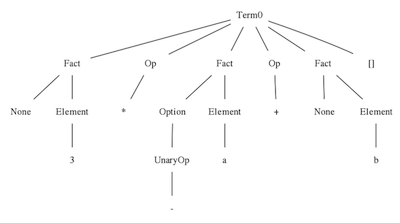
\includegraphics[width=4in]{./examples/ebnf/arith/ebnf-arith.png}
  \caption{Syntax Tree for\\ \textit{3 * -a + b}}
\end{figure}



